%-------------------------------------------------------------------
% Standalone summary: Experiments and results
% Compile from thesis-latex: pdflatex experiments_summary
%-------------------------------------------------------------------
\documentclass[11pt,a4paper]{article}
\usepackage[utf8]{inputenc}
\usepackage[T1]{fontenc}
\usepackage[english]{babel}
\usepackage{lmodern}
\usepackage{geometry}
\geometry{margin=2.5cm}
\usepackage{graphicx}
\usepackage{booktabs}
\usepackage{amsmath}
\usepackage{hyperref}
\usepackage{parskip}
\usepackage{caption}
\captionsetup{labelfont=bf}

\title{Summary: MNCA Experiments and Results}
\author{}
\date{}

\begin{document}
\maketitle
\tableofcontents
\newpage

%-------------------------------------------------------------------
\section{Introduction}
%-------------------------------------------------------------------

We ask whether increasing the neighborhood size \(NB\) in Mixture Neural Cellular Automata (MNCA) improves long-horizon behaviour in a tissue-growth setup. Experiments are run as a sequence of controlled studies. The main one is Step~3: we train models with \(NB \in \{1,\dots,7\}\) on 300 trajectories of 100 steps and evaluate at rollout lengths 25, 50, and 100.

%-------------------------------------------------------------------
\section{Why Step~3}
%-------------------------------------------------------------------

We started from the MNCA paper setup (small data, short horizon). Varying only \(NB\) did not give a clear answer: rollouts were unstable and metric gaps small. We then tried more data (1000 trajectories, 500 steps) and curriculum learning; training was slow and results mixed, so the effect of \(NB\) was hard to see when models were already failing.

Step~3 fixes this: we keep sampling and temperature fixed, use 300 trajectories of 100 steps, and evaluate at several horizons. This makes the effect of \(NB\) visible (e.g.\ slower decay and better stability when we lengthen the rollout).

%-------------------------------------------------------------------
\section{Evaluation and main trends}
%-------------------------------------------------------------------

We use six metrics on the final state of each run. All are ``lower is better''. Below we state on what each one is computed.

\subsection{What each metric is computed on}
\label{sec:metrics-def}

\textbf{Evaluation data.} Each evaluation uses \(N\) simulations (in our runs, \(N=300\)). For each simulation \(i\) we have: the same initial grid, the \emph{true} final state (from the ground-truth simulator) and the \emph{generated} final state (from the model, same initial condition). So we have \(N\) true final grids and \(N\) generated final grids, in one-to-one correspondence (simulation \(i\) gives true grid \(i\) and generated grid \(i\)). Each grid is 2D with one cell type per site (e.g.\ STEM, INTERMEDIATE, DIFFERENTIATED, EMPTY). All six metrics compare these two sets of \(N\) grids; below we say exactly on what data each metric is built and what ``distribution'' means when we use that word.

\paragraph{KL divergence.} \emph{Data:} we pool all cells from all \(N\) true grids into one multiset, and all cells from all \(N\) generated grids into another. So we ignore which simulation or which site each cell comes from; we only keep the cell type. \emph{Distributions:} we count how many cells of each type (excluding EMPTY) there are in the pooled true multiset and in the pooled generated multiset, then we normalize to get two probability vectors over the set of cell types. So we get one distribution for ``true'' and one for ``generated'', each on the same set of types. \emph{Metric:} KL divergence \(\sum p\,\log(p/q)\) between these two vectors. It measures how well the global mix of cell types in the generated set matches the true set, with no spatial or per-simulation structure.

\paragraph{Chi-square.} \emph{Data and distributions:} exactly the same as for KL: the two probability vectors over cell types from the pooled true and pooled generated cells. \emph{Metric:} \(\sum (p-q)^2/(p+q)\). Same level of information as KL (global cell-type proportions only).

\paragraph{Categorical MMD.} \emph{Data:} the \(N\) true grids and the \(N\) generated grids, each kept as a full 2D pattern (we do not pool or aggregate). So each ``point'' is one entire grid. \emph{No distribution over simulations:} we do not build an empirical distribution of a scalar; we compare two sets of objects. \emph{Metric:} we use a kernel that, given two grids, counts how often the cell type matches position by position, and we form the usual MMD: \(\mathrm{mean}(k_{\mathrm{true,true}}) + \mathrm{mean}(k_{\mathrm{gen,gen}}) - 2\,\mathrm{mean}(k_{\mathrm{true,gen}})\). So we measure how similar the spatial layouts of cell types are between the two sets of grids, using the full pattern of each grid.

\paragraph{Tumor size difference.} \emph{Data:} for each simulation \(i\) we compute one number from the true grid (count of non-empty cells) and one from the generated grid (same quantity). So we have two lists of \(N\) numbers: \((\text{tumor size of true grid}_1,\dots)\) and \((\text{tumor size of generated grid}_1,\dots)\). \emph{Distributions:} we treat each list as an empirical distribution over the \(N\) simulations. So ``true distribution'' = the empirical distribution of tumor size across the \(N\) true grids; ``generated distribution'' = the empirical distribution of tumor size across the \(N\) generated grids. \emph{Metric:} Wasserstein distance between these two empirical distributions, normalized by the mean of the true tumor sizes. So we ask whether the spread of total cell counts over simulations in the generated set is similar to that in the true set.

\paragraph{Border size difference.} \emph{Data:} for each grid we compute ``border size'' (see below); so we get one number per true grid and one per generated grid, i.e.\ two lists of \(N\) numbers. \emph{Distributions:} again, the empirical distributions of these \(N\) values for true and for generated. \emph{Metric:} Wasserstein distance between these two distributions, normalized by the mean true border size. Border size itself is computed per grid as follows: we build a binary mask (1 where there is any non-empty cell, 0 at EMPTY), apply a 3\(\times\)3 edge-detection kernel (Laplacian-like), and count pixels with strong response---that is the length of the tissue--empty interface for that grid. So we compare the distribution of ``perimeter length'' over the \(N\) simulations.

\paragraph{Spatial variance difference.} \emph{Data:} for each grid we compute ``spatial variance'' (see below), giving two lists of \(N\) numbers. \emph{Distributions:} the empirical distributions of these \(N\) values for true and for generated. \emph{Metric:} Wasserstein distance between these two distributions, normalized by the mean true spatial variance. Spatial variance per grid is: take the positions of all non-empty cells, compute their centre of mass, then the mean squared distance of those cells from that centre. So we compare the distribution of ``spread around the centre'' over the \(N\) simulations.

\medskip
\noindent\textit{Summary.} KL and Chi-square use \emph{pooled} data (all cells from all \(N\) grids merged) and compare two distributions \emph{over cell types}. Categorical MMD uses the \(N\) full grids as objects and compares two sets via a kernel (no scalar distribution). Tumor size, border size, and spatial variance each compute one scalar per grid, so we have two lists of \(N\) numbers; the ``distributions'' are the empirical distributions of that scalar over the \(N\) simulations, and we compare them with (normalized) Wasserstein distance.

%-------------------------------------------------------------------
\subsection{Metrics dashboard}
%-------------------------------------------------------------------

\begin{figure}[htbp]
  \centering
  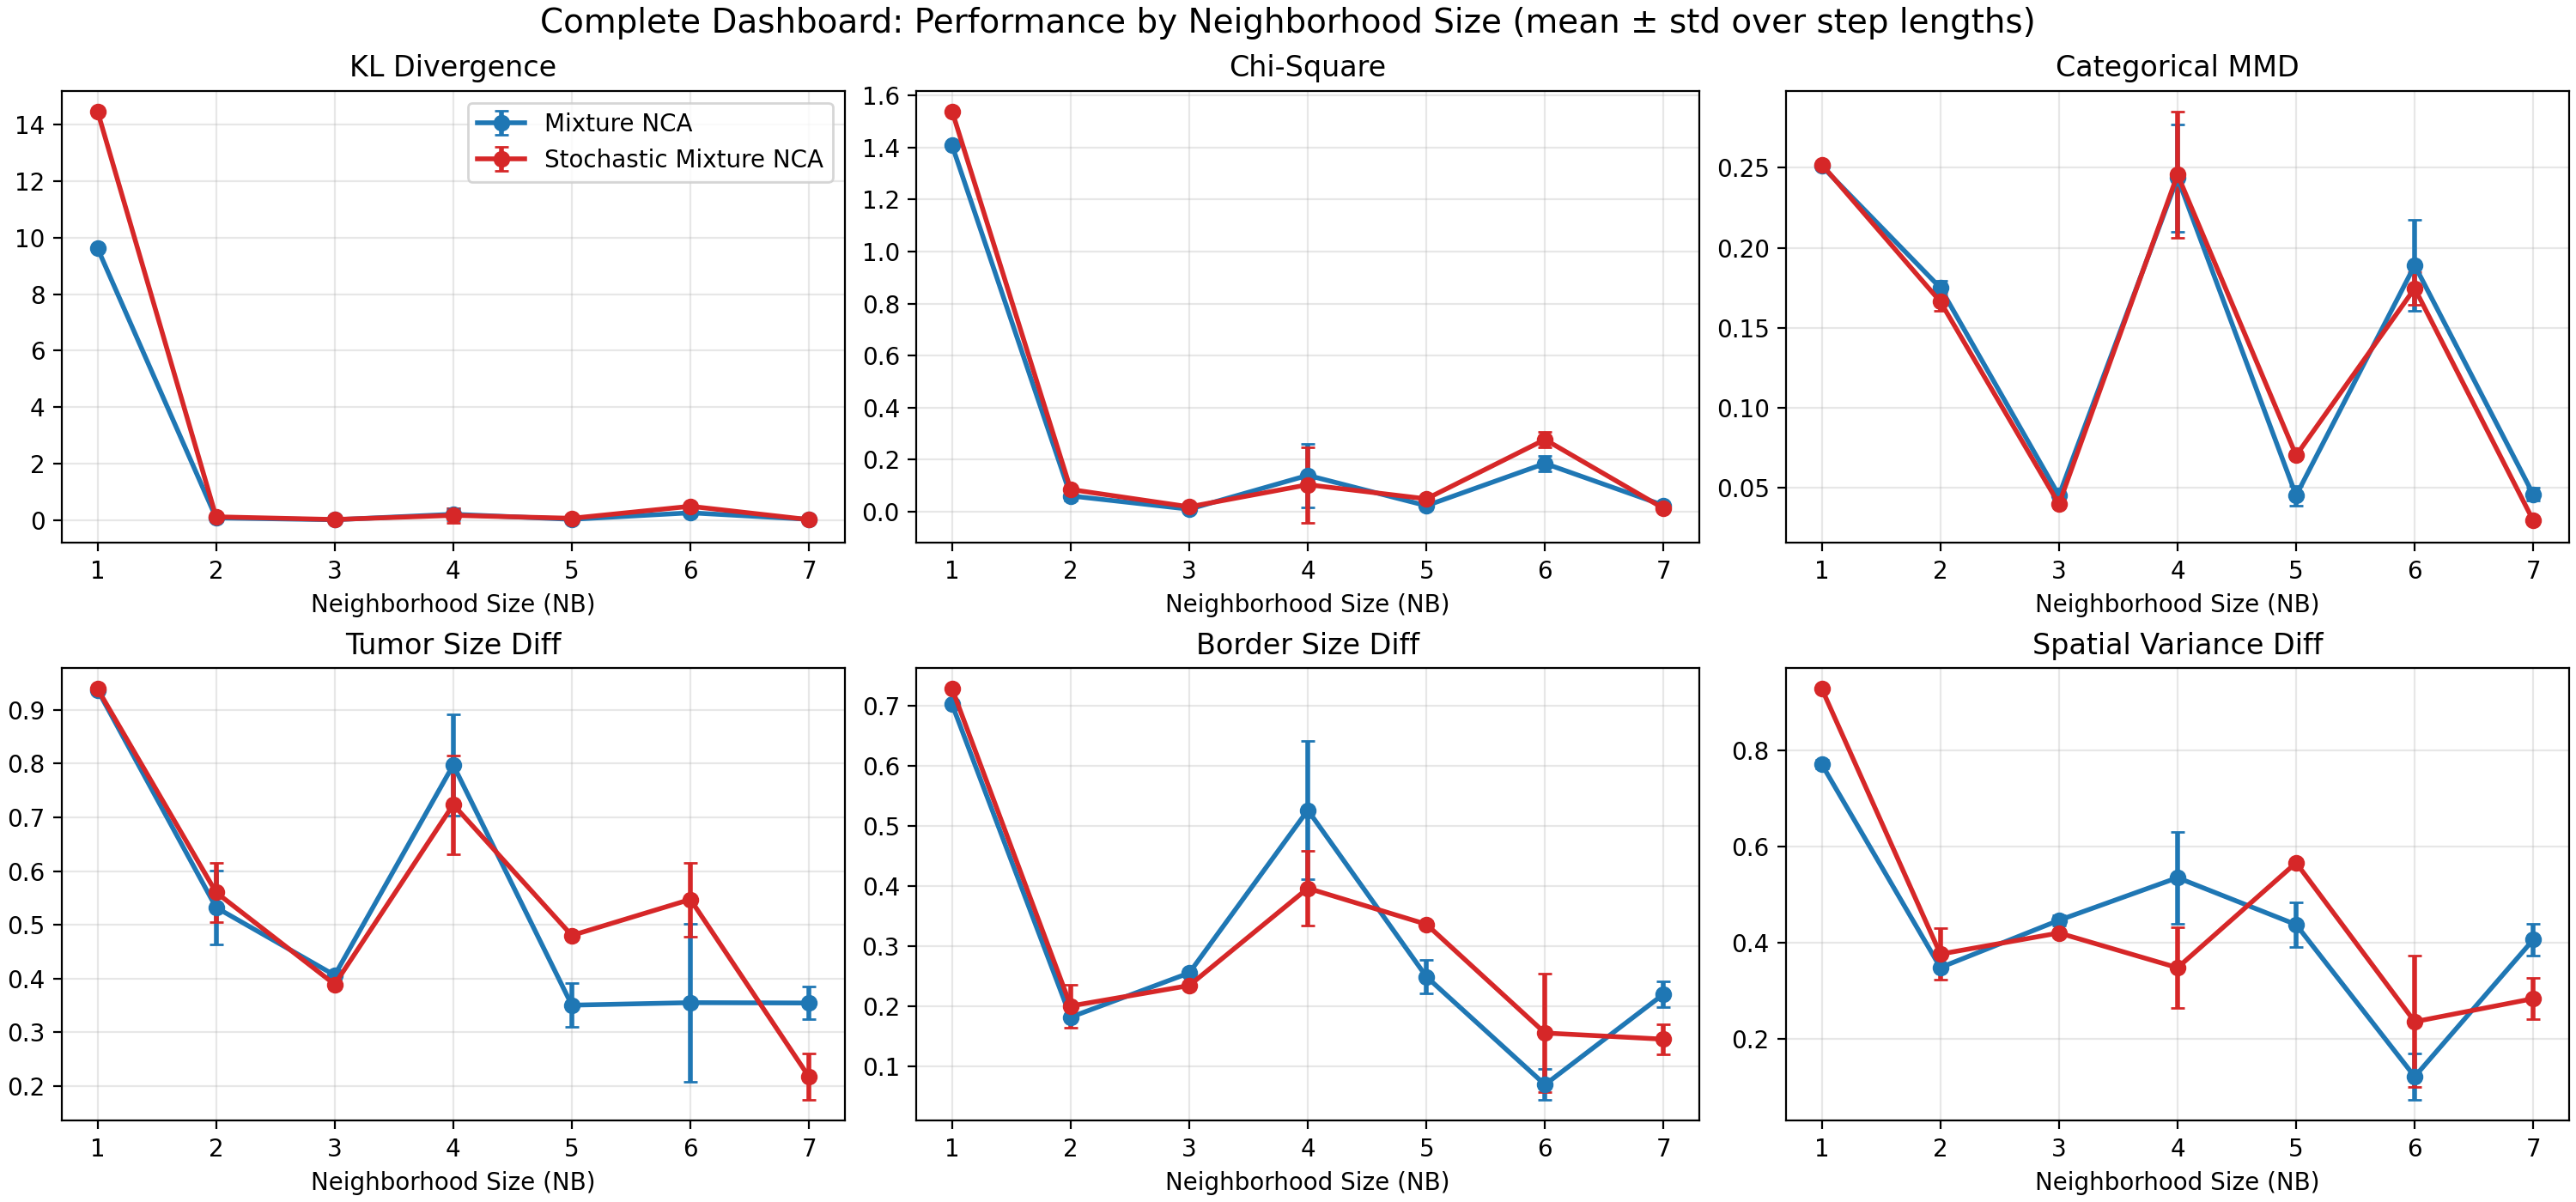
\includegraphics[width=\textwidth]{figs/neighborhood_analysis/nb_sweep_300x100/metrics_dashboard_full.png}
  \caption{Mean and spread over step-length conditions for all six metrics.}
  \label{fig:dashboard}
\end{figure}

\textbf{Interpretation.} \(NB=1\) is clearly worse than \(NB\ge2\); moving from 1 to 2 gives a big gain. For \(NB\ge2\), scores do not keep improving as \(NB\) grows. The best \(NB\) depends on the metric and on rollout length. Mixture and Stochastic Mixture can behave differently. Distribution metrics (KL, Chi-square, MMD) and spatial ones (tumor size, border, variance) often tell a similar story for \(NB=1\) vs.\ \(NB\ge2\), but they can disagree on which \(NB\ge2\) is best---e.g.\ one \(NB\) can match global cell-type counts well while another fits border shape better.

%-------------------------------------------------------------------
\section{Per-simulation variability (violins)}
%-------------------------------------------------------------------

Averages can hide bad runs. Violin plots show the full distribution per \(NB\) and step length.

\begin{figure}[htbp]
  \centering
  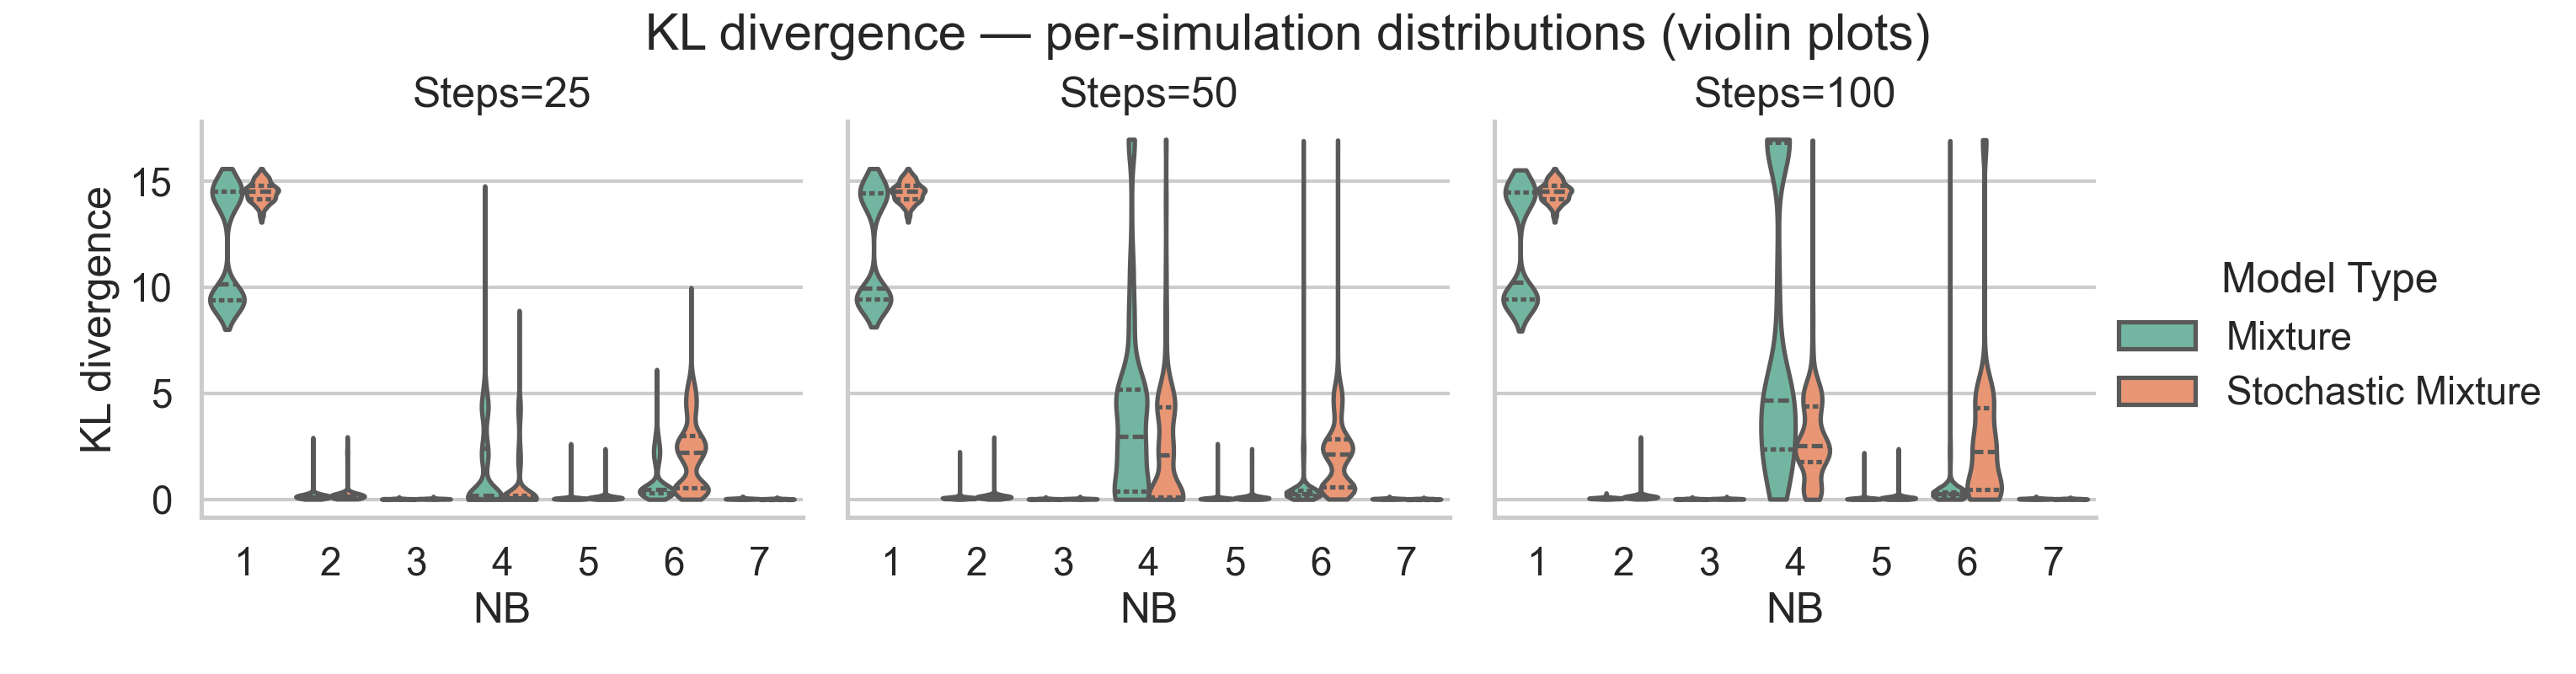
\includegraphics[width=\textwidth]{figs/neighborhood_analysis/nb_sweep_300x100/violin_KL_Divergence.png}
  \caption{KL divergence per run (lower is better). Wide part = density; long upper tail = many bad runs.}
  \label{fig:violin:kl}
\end{figure}

\textbf{Interpretation.} \(NB=1\) has very high KL and long upper tails. With \(NB\ge2\), the bulk improves and tails shorten. So \(NB\ge2\) is needed for stable rollouts that match the target distribution. At longer step lengths (e.g.\ 100) the violins often spread out more, so the gain of \(NB\ge2\) is easier to see when we push the rollout length.

\begin{figure}[htbp]
  \centering
  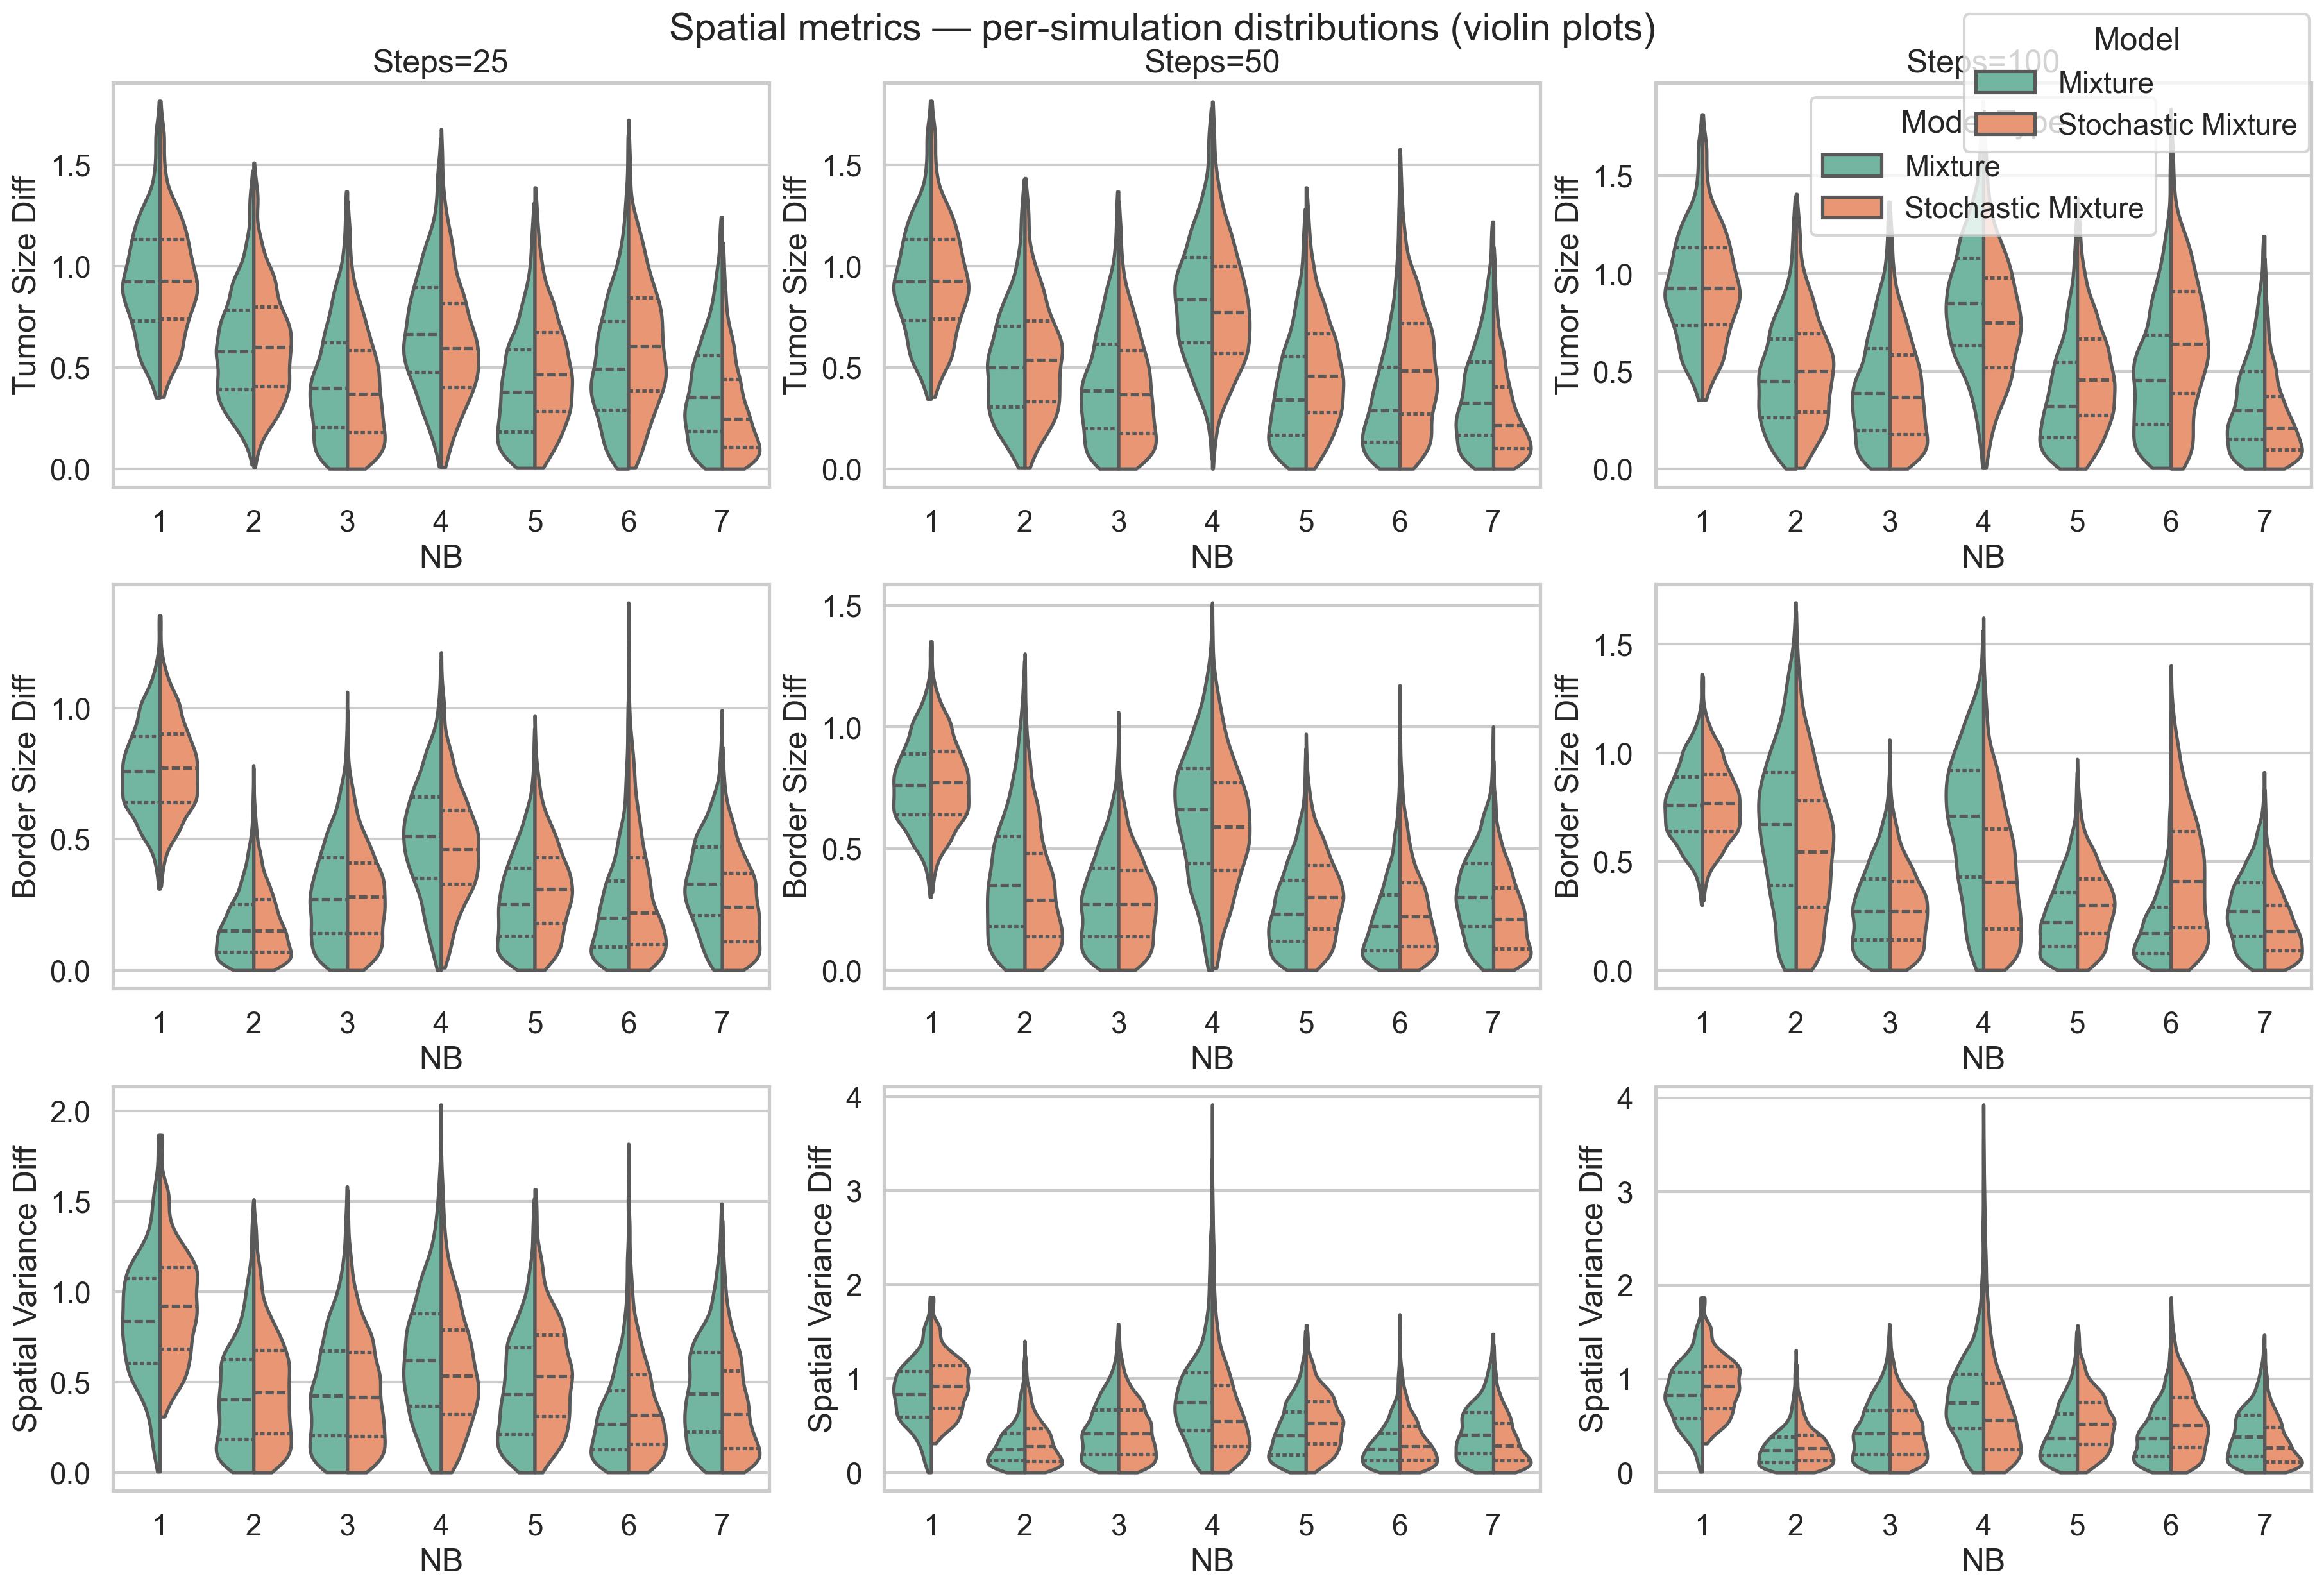
\includegraphics[width=\textwidth]{figs/neighborhood_analysis/nb_sweep_300x100/violin_spatial_metrics.png}
  \caption{Spatial metrics per run (tumor size, border size, spatial variance; lower is better).}
  \label{fig:violin:spatial}
\end{figure}

\textbf{Interpretation.} Same idea: \(NB=1\) is bad, \(NB\ge2\) is better. Spread and tails depend on \(NB\) and step length; longer rollouts make the differences between \(NB\) clearer. Tumor size and border size show which \(NB\) keep mass and shape under control; spatial variance picks up how patchy or smooth the pattern is, and some \(NB\) do better on that than others.

%-------------------------------------------------------------------
\section{Fold change (NB=7 vs NB=3)}
%-------------------------------------------------------------------

\begin{figure}[htbp]
  \centering
  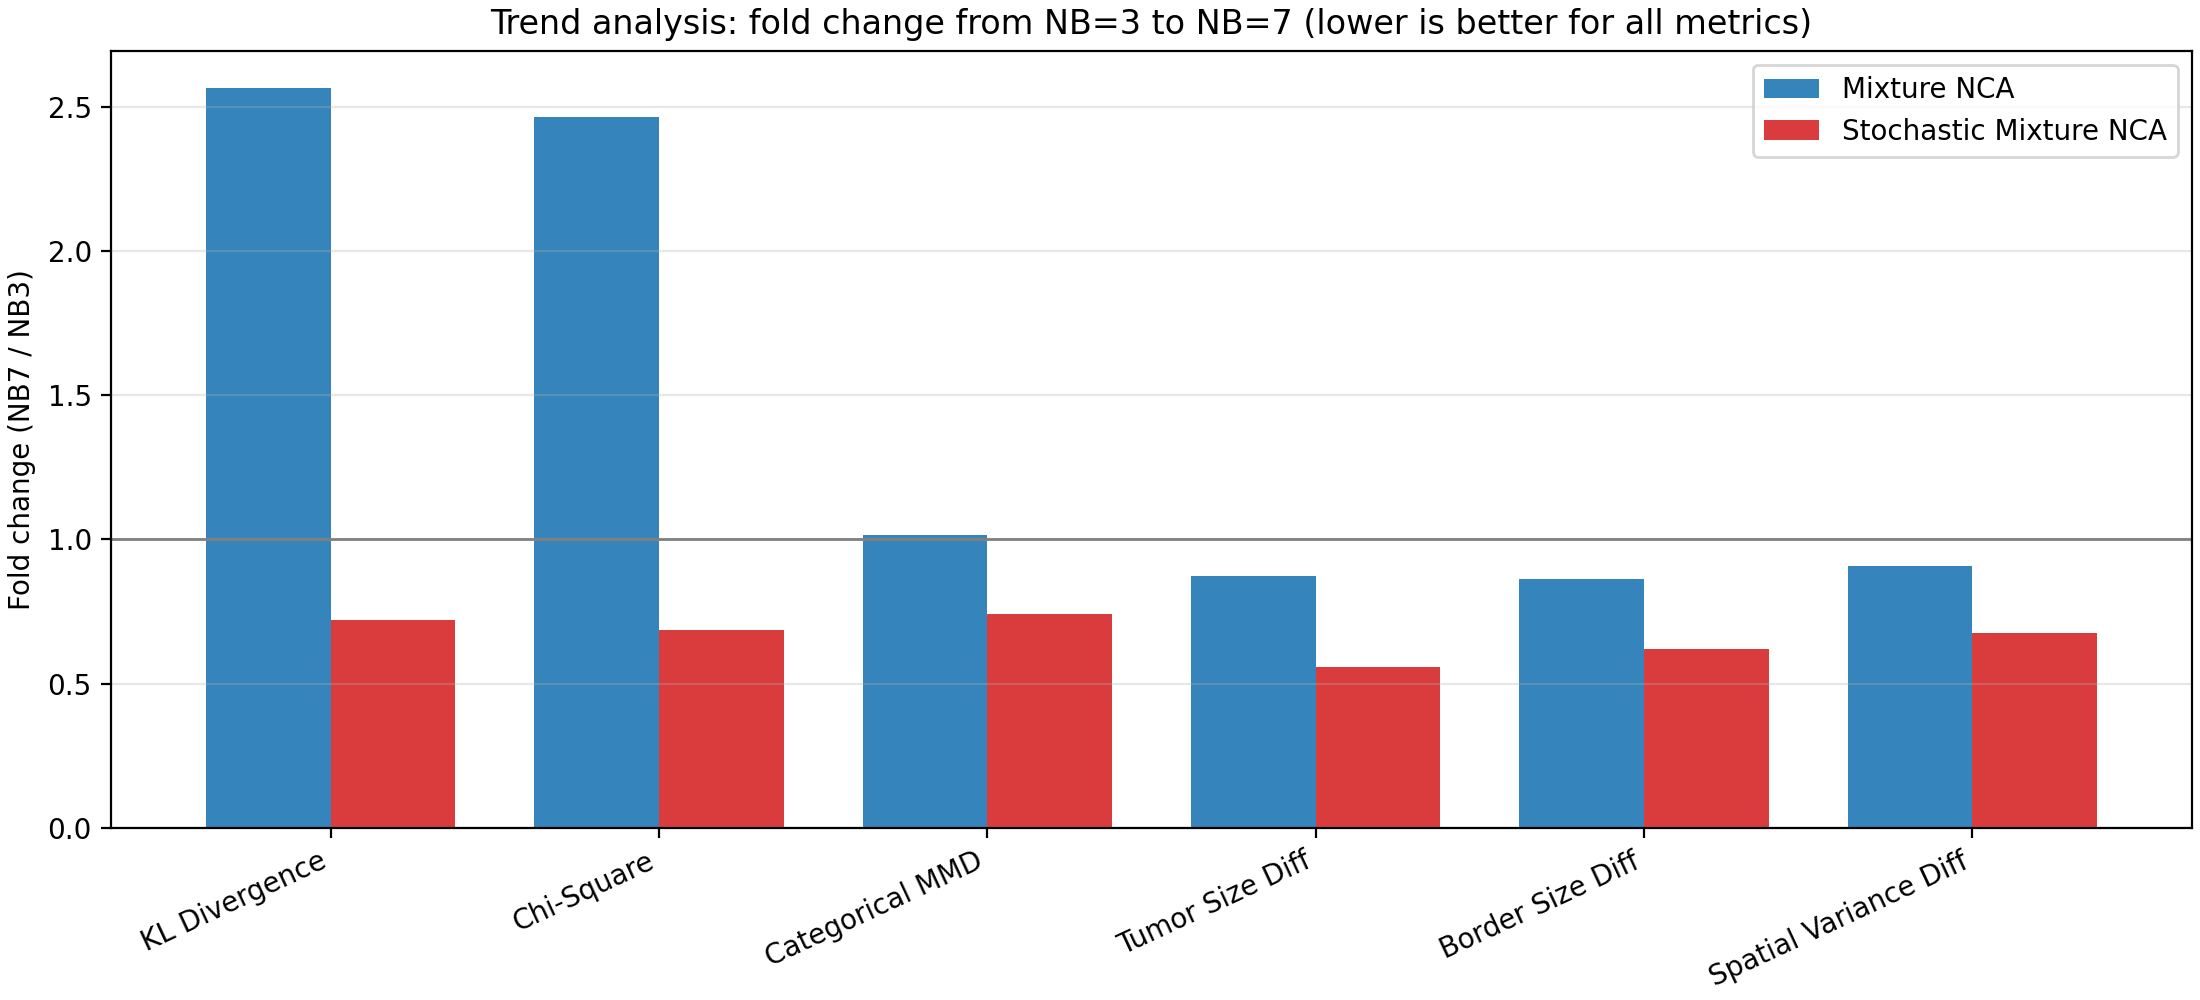
\includegraphics[width=\textwidth]{figs/neighborhood_analysis/nb_sweep_300x100/trend_foldchange_nb7_over_nb3.png}
  \caption{Ratio metric(\(NB{=}7\))/metric(\(NB{=}3\)). Below 1 = better at \(NB{=}7\); above 1 = worse.}
  \label{fig:foldchange}
\end{figure}

\textbf{Interpretation.} The main jump is from \(NB=1\) to \(NB\ge2\). Among \(NB\ge2\), differences are smaller and depend on the metric. Going from \(NB=3\) to \(NB=7\) often gives ratios near or above 1, so increasing \(NB\) from 3 to 7 does not always help and can hurt some metrics. Which metric improves or worsens with larger \(NB\) can differ between Mixture and Stochastic Mixture, so the fold-change plot is a quick way to see where the two models agree or disagree.

%-------------------------------------------------------------------
\section{Bad-rate (robustness)}
%-------------------------------------------------------------------

Bad-rate = share of runs whose metric is worse than the 95th percentile of the best \(NB\) (for that model and step length). Low bad-rate = fewer severe failures.

\begin{figure}[htbp]
  \centering
  
\includegraphics[width=\textwidth]{figs/neighborhood_analysis/nb_sweep_300x100/badrate_bars_KL_Divergence.png}
  \caption{Bad-rate for KL (lower is better).}
  \label{fig:badrate:kl}
\end{figure}

\textbf{Interpretation.} \(NB=1\) has high bad-rate; \(NB\ge2\) lowers it. Some \(NB\ge2\) still have high bad-rate at certain step lengths. So even when the mean KL looks good, a non-negligible share of runs can still end up with wrong cell-type distributions---the bars show which \(NB\) and which step length reduce that share the most.

\begin{figure}[htbp]
  \centering
  
\includegraphics[width=\textwidth]{figs/neighborhood_analysis/nb_sweep_300x100/badrate_bars_Tumor_Size_Diff.png}
  \caption{Bad-rate for tumor size (lower is better).}
  \label{fig:badrate:tumor}
\end{figure}

\textbf{Interpretation.} Bad-rate drops from \(NB=1\) to \(NB\ge2\). For the stochastic model, larger \(NB\) often reduces it further. Tumor size bad-rate is about getting the overall mass right; when it is high, many runs end up with too small or too large a ``tumor'', and the plot shows which \(NB\) fix that.

\begin{figure}[htbp]
  \centering
  
\includegraphics[width=\textwidth]{figs/neighborhood_analysis/nb_sweep_300x100/badrate_bars_Border_Size_Diff.png}
  \caption{Bad-rate for border size (lower is better).}
  \label{fig:badrate:border}
\end{figure}

\textbf{Interpretation.} Border bad-rate depends on \(NB\) and step length. Some \(NB\) have many runs with bad borders even when the median is OK. Border size tracks the interface between tissue and empty space; when this goes wrong, the pattern often looks too smooth or too ragged compared to the target, and the bad-rate bars show where that happens most.

\begin{figure}[htbp]
  \centering
  
\includegraphics[width=\textwidth]{figs/neighborhood_analysis/nb_sweep_300x100/badrate_bars_Spatial_Variance_Diff.png}
  \caption{Bad-rate for spatial variance (lower is better).}
  \label{fig:badrate:spvar}
\end{figure}

\textbf{Interpretation.} Spatial variance is sensitive to \(NB\) and horizon. Looking at both the center and the tails helps see when larger \(NB\) helps. Spatial variance bad-rate picks up runs where the local variability of the pattern (e.g.\ how mixed or segregated cell types are) is far from the target; the plot shows which \(NB\) and step lengths keep that under control.

%-------------------------------------------------------------------
\section{Compute and rule use}
%-------------------------------------------------------------------

\subsection{Runtime}

\begin{figure}[htbp]
  \centering
  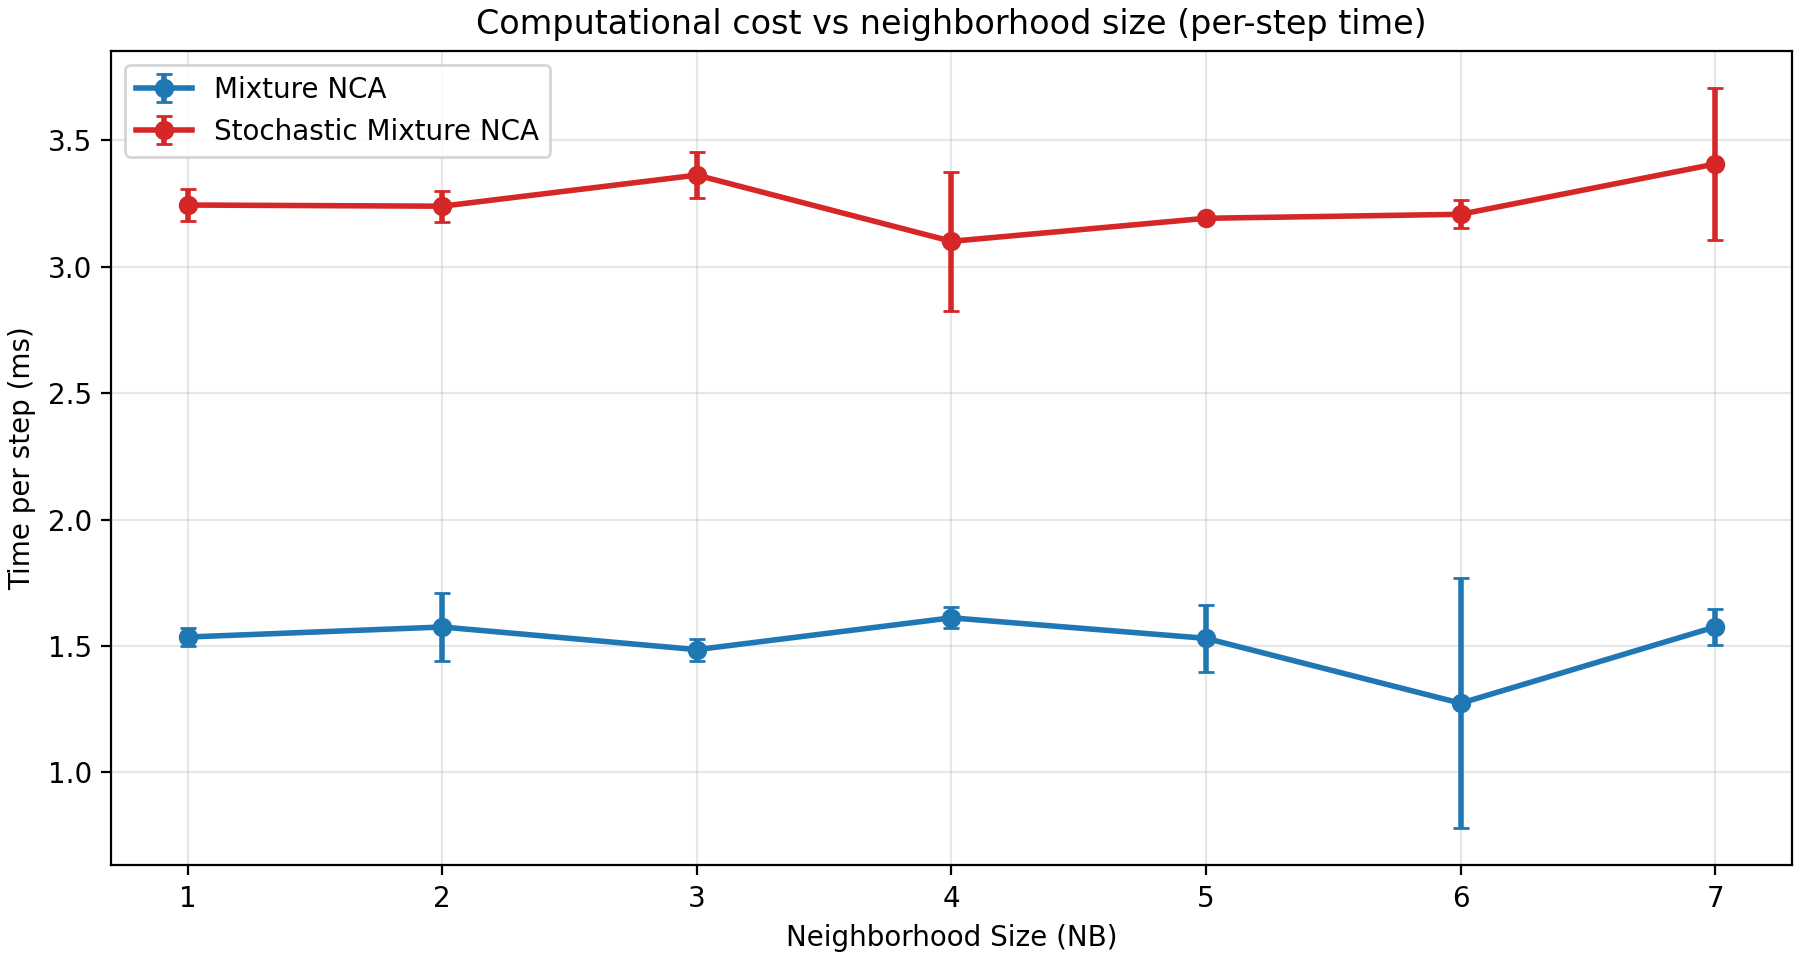
\includegraphics[width=0.9\textwidth]{figs/neighborhood_analysis/nb_sweep_300x100/computational_complexity_time_per_step.png}
  \caption{Time per step (ms) vs.\ \(NB\).}
  \label{fig:complexity:time}
\end{figure}

\textbf{Interpretation.} For \(NB\in[1,7]\), runtime is almost flat (Mixture ~1.5\,ms/step, Stochastic ~3.2\,ms/step). Cost is dominated by constants, not by \(NB^2\), so using larger \(NB\) in this range adds little cost. The Stochastic variant is about twice as slow per step because it samples rules; both curves stay roughly flat, so we are not paying a big price for going from \(NB=3\) to \(NB=7\).

\begin{figure}[htbp]
  \centering
  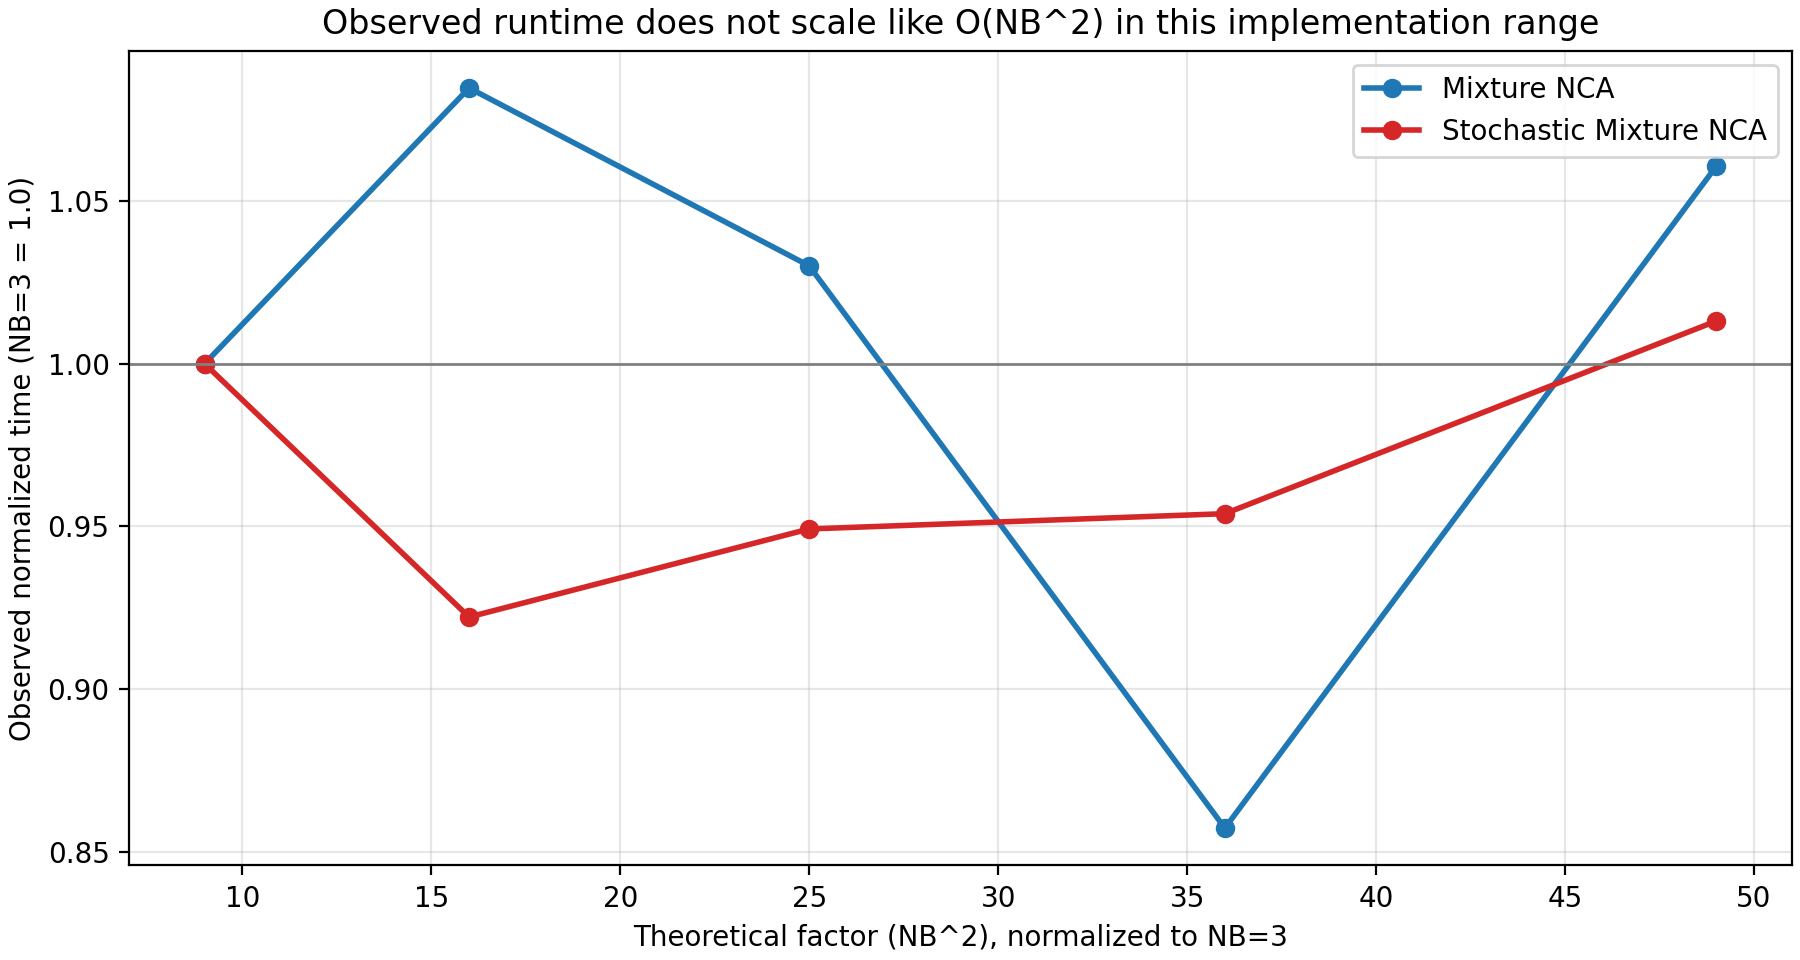
\includegraphics[width=0.9\textwidth]{figs/neighborhood_analysis/nb_sweep_300x100/computational_complexity_normalized_vs_theory.png}
  \caption{Normalized time vs.\ \(NB=3\). It stays near 1.0; no clear \(NB^2\) growth.}
  \label{fig:complexity:theory}
\end{figure}

\textbf{Interpretation.} Normalized runtime stays close to 1.0, so we do not see quadratic growth with \(NB\) in practice. If cost scaled like \(NB^2\), the normalized curve would rise as we increase \(NB\); the flat profile means that in this range the implementation (e.g.\ vectorization, fixed overhead) hides the naive scaling.

\subsection{Rule entropy over time}

\begin{figure}[htbp]
  \centering
  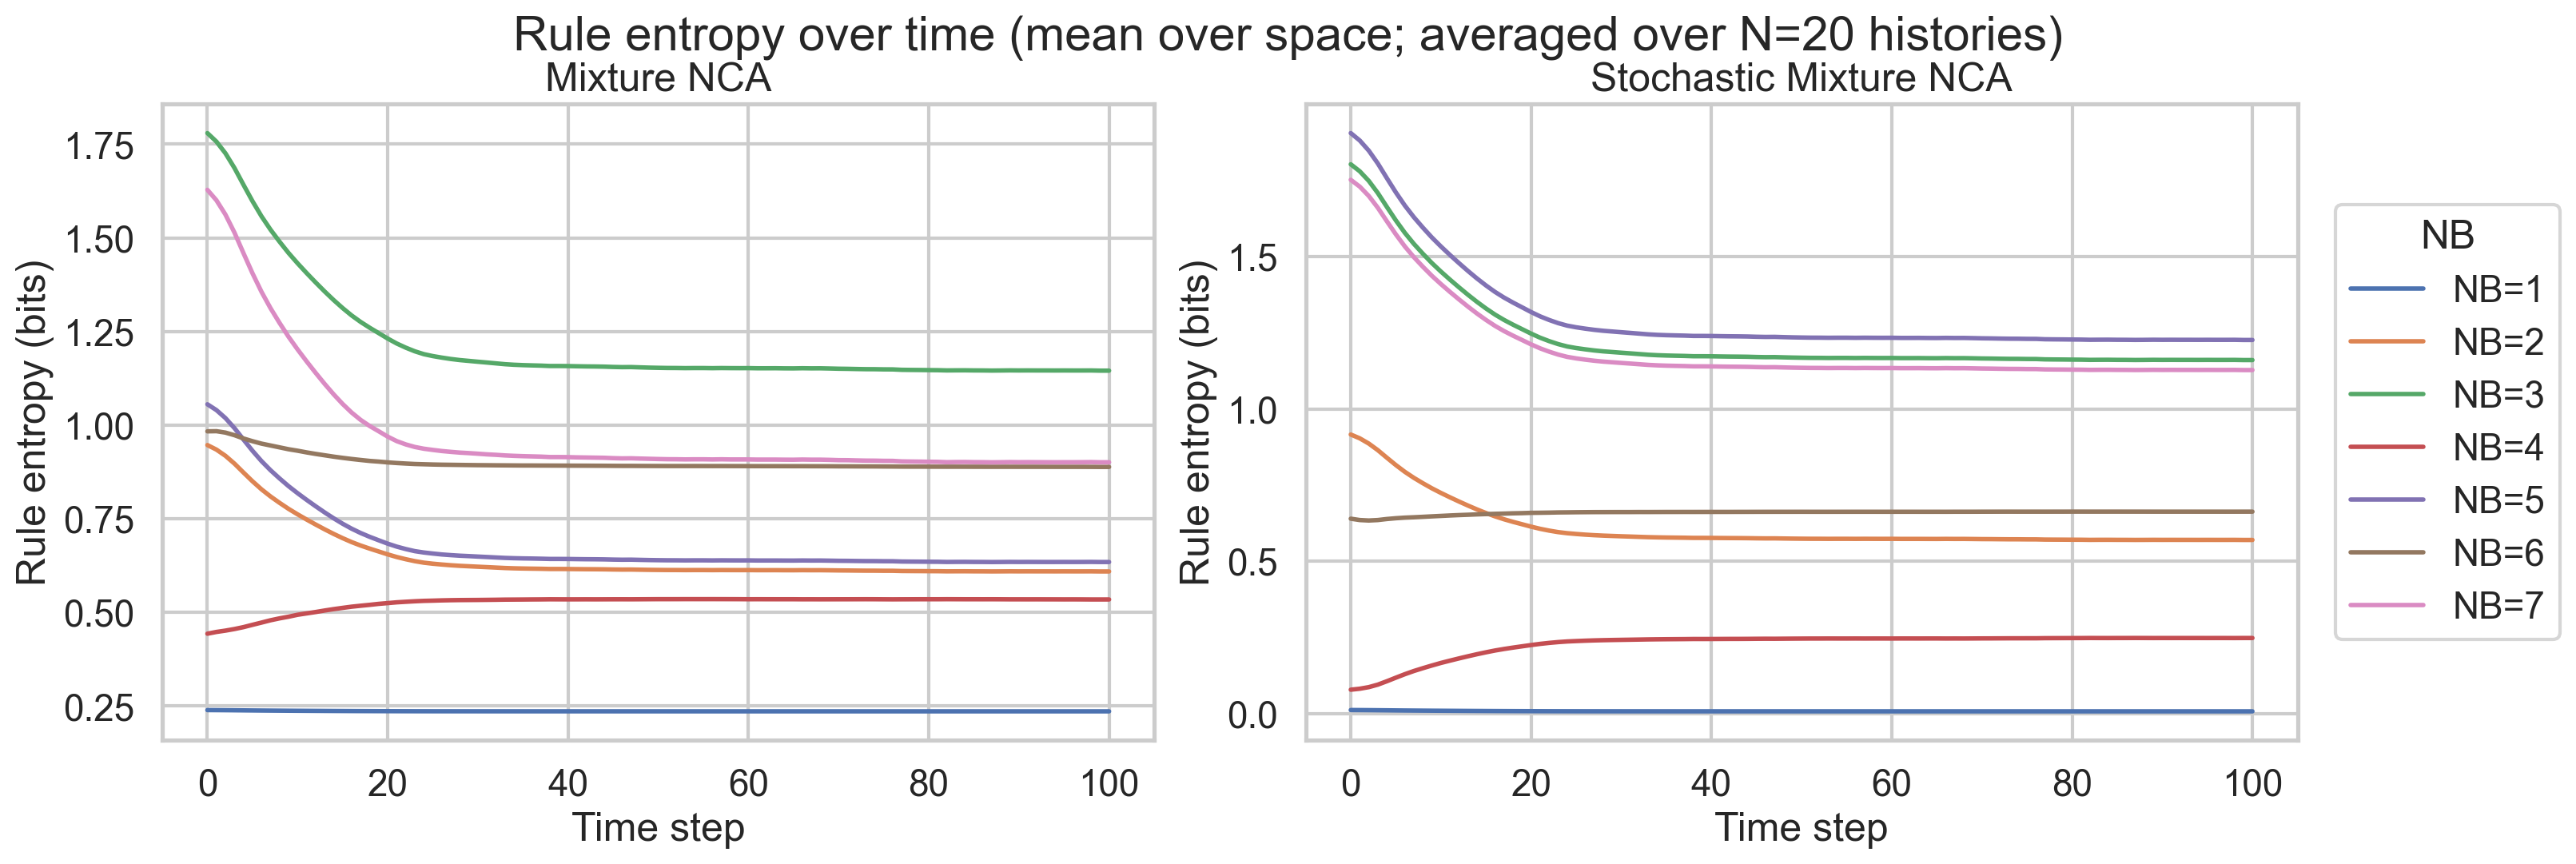
\includegraphics[width=\textwidth]{figs/neighborhood_analysis/nb_sweep_300x100/rule_entropy_over_time.png}
  \caption{Entropy of rule assignment over time (bits). Lower = more confident rule choice.}
  \label{fig:entropy:time}
\end{figure}

\textbf{Interpretation.} Entropy shows how the model picks rules over time. Larger \(NB\) can change this path and match the stability and metric differences we see across \(NB\). For example, some \(NB\) may show a fast drop in entropy (the model quickly commits to a few rules), while others keep entropy higher for longer; that can go together with more or fewer failure modes in the metrics.

\subsection{Rule specialization summary}

\begin{figure}[htbp]
  \centering
  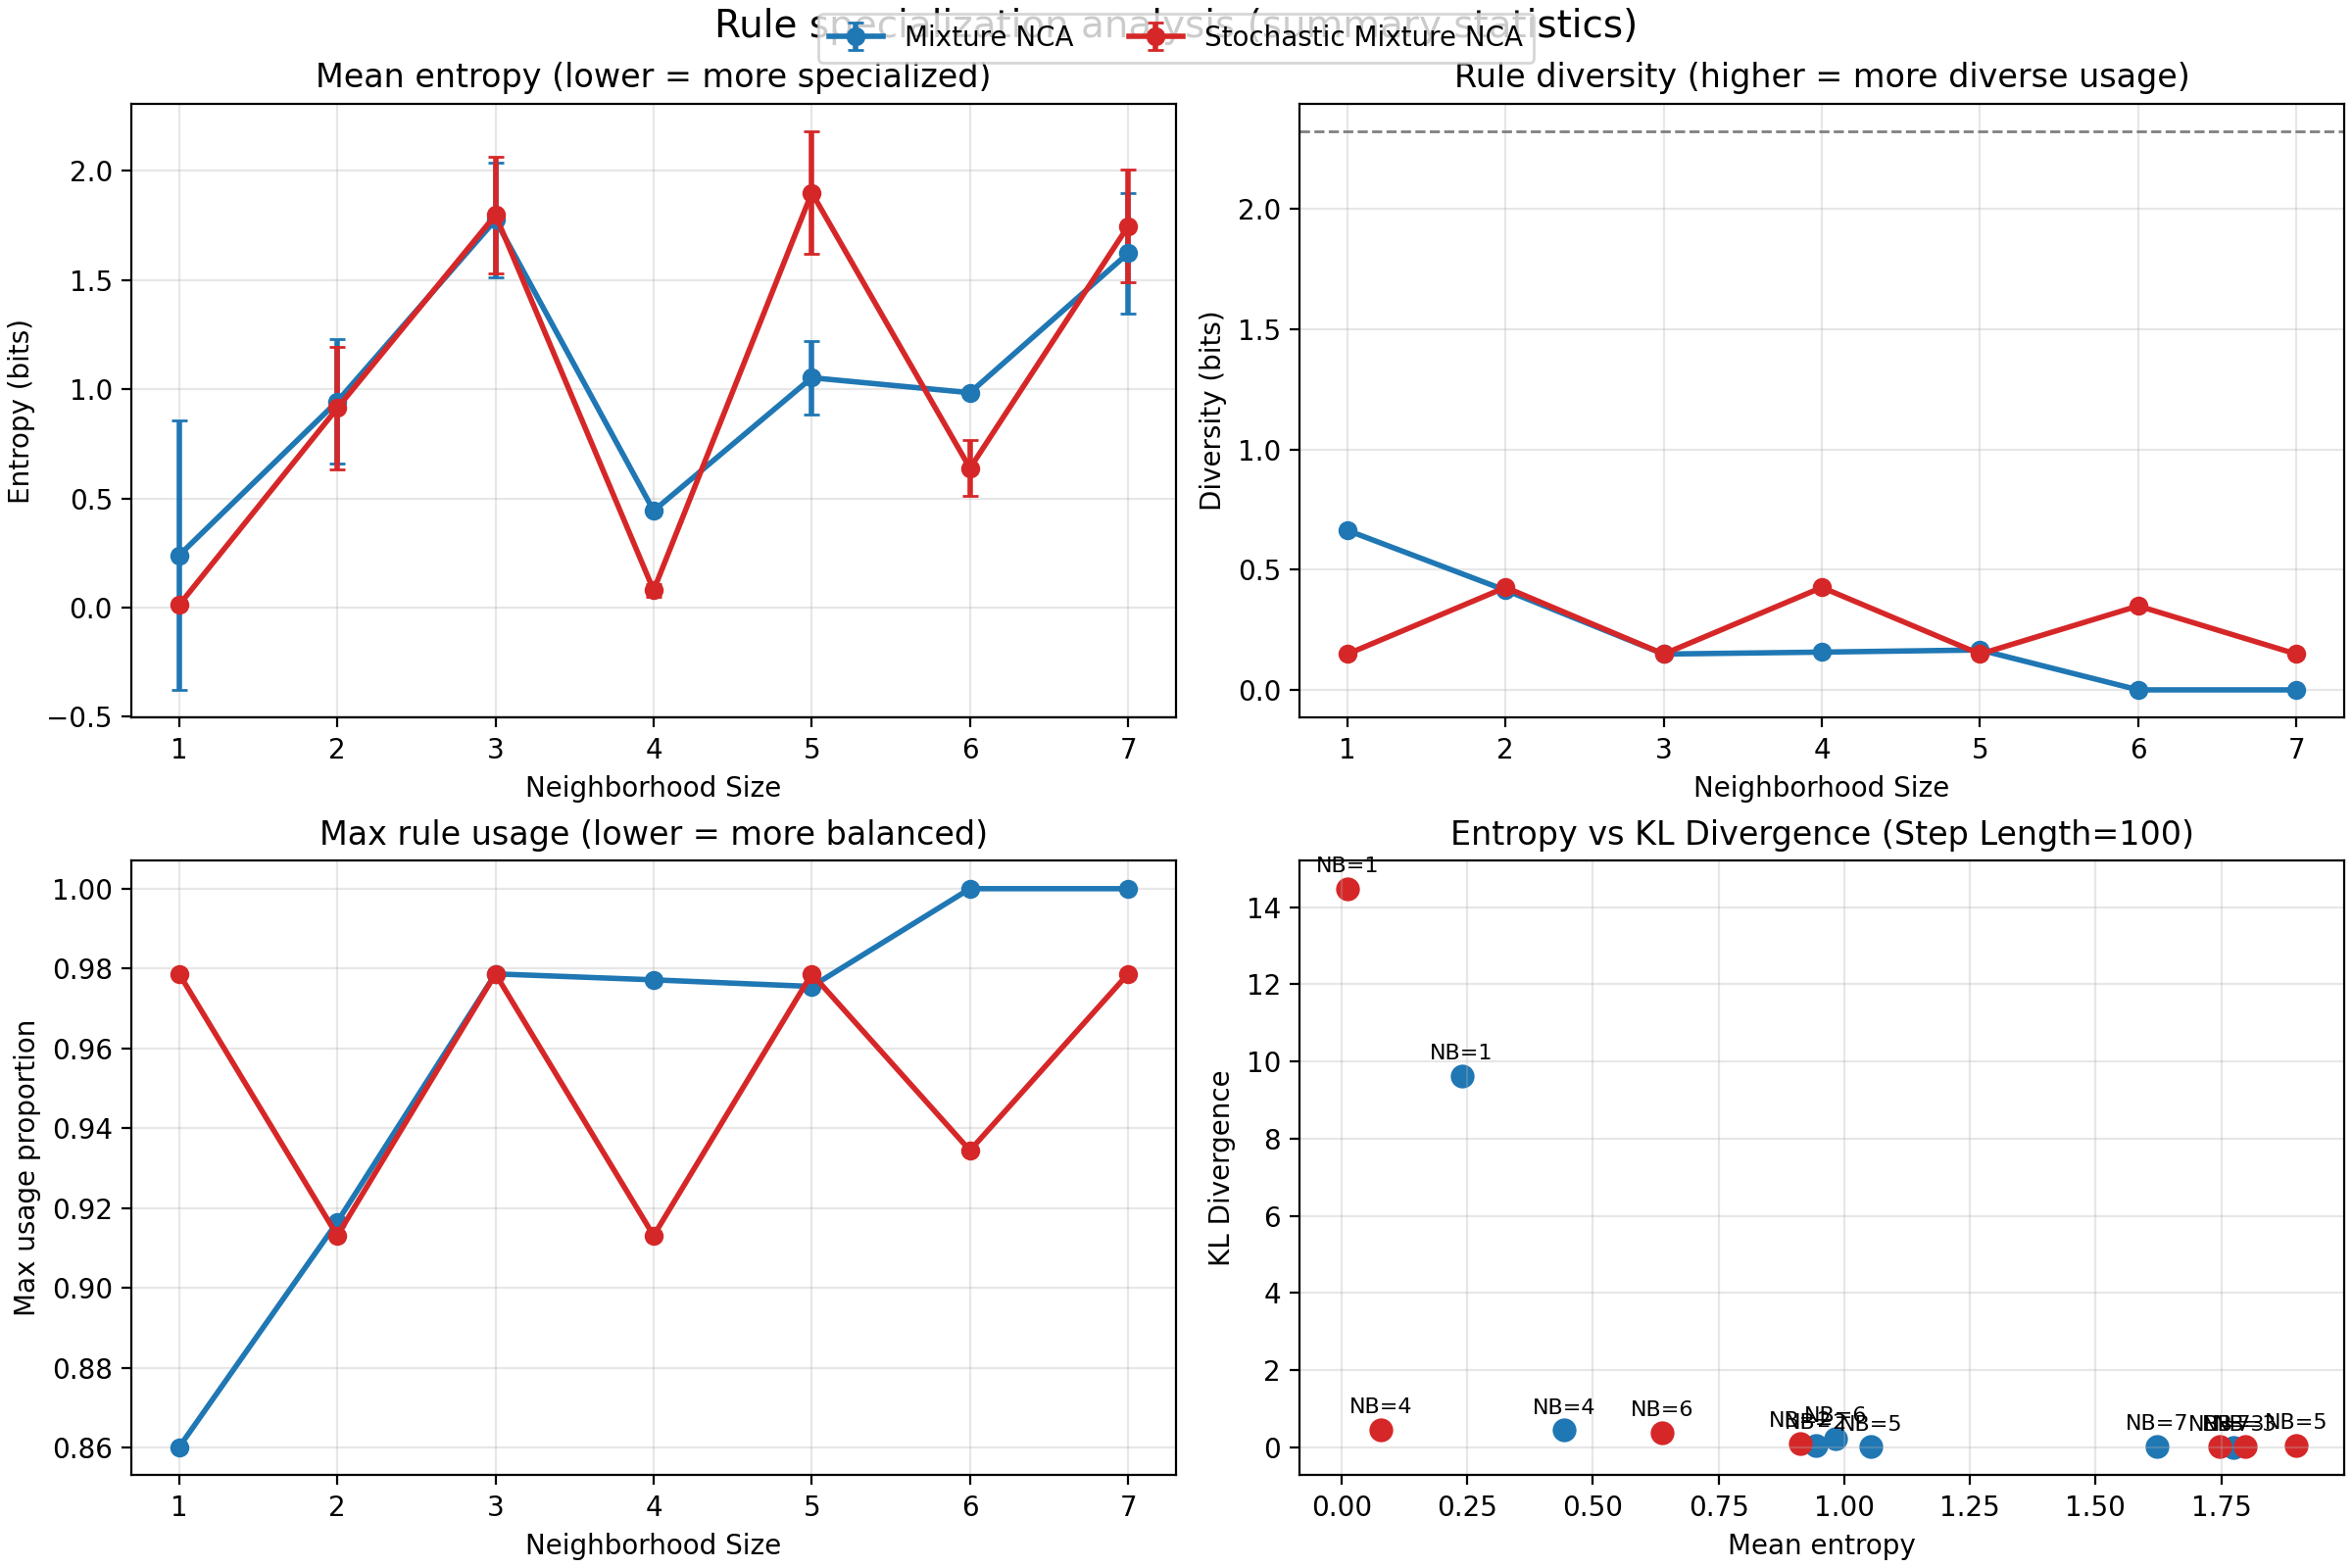
\includegraphics[width=\textwidth]{figs/neighborhood_analysis/nb_sweep_300x100/rule_specialization_summary.png}
  \caption{Summary of rule use (entropy, diversity, max rule share) and link to KL at step length 100.}
  \label{fig:rule:summary}
\end{figure}

\textbf{Interpretation.} Rule use varies with \(NB\). More confident or more balanced rule use does not always give the best KL; it depends on metric and horizon. The panel that links entropy (or other specialization indices) to KL at step length 100 lets us check whether ``more specialized'' tends to mean ``better'' or not---often there is no single trend, which fits with the idea that different \(NB\) trade off distribution match and spatial structure in different ways.

\subsection{Rule-assignment maps}

\begin{figure}[htbp]
  \centering
  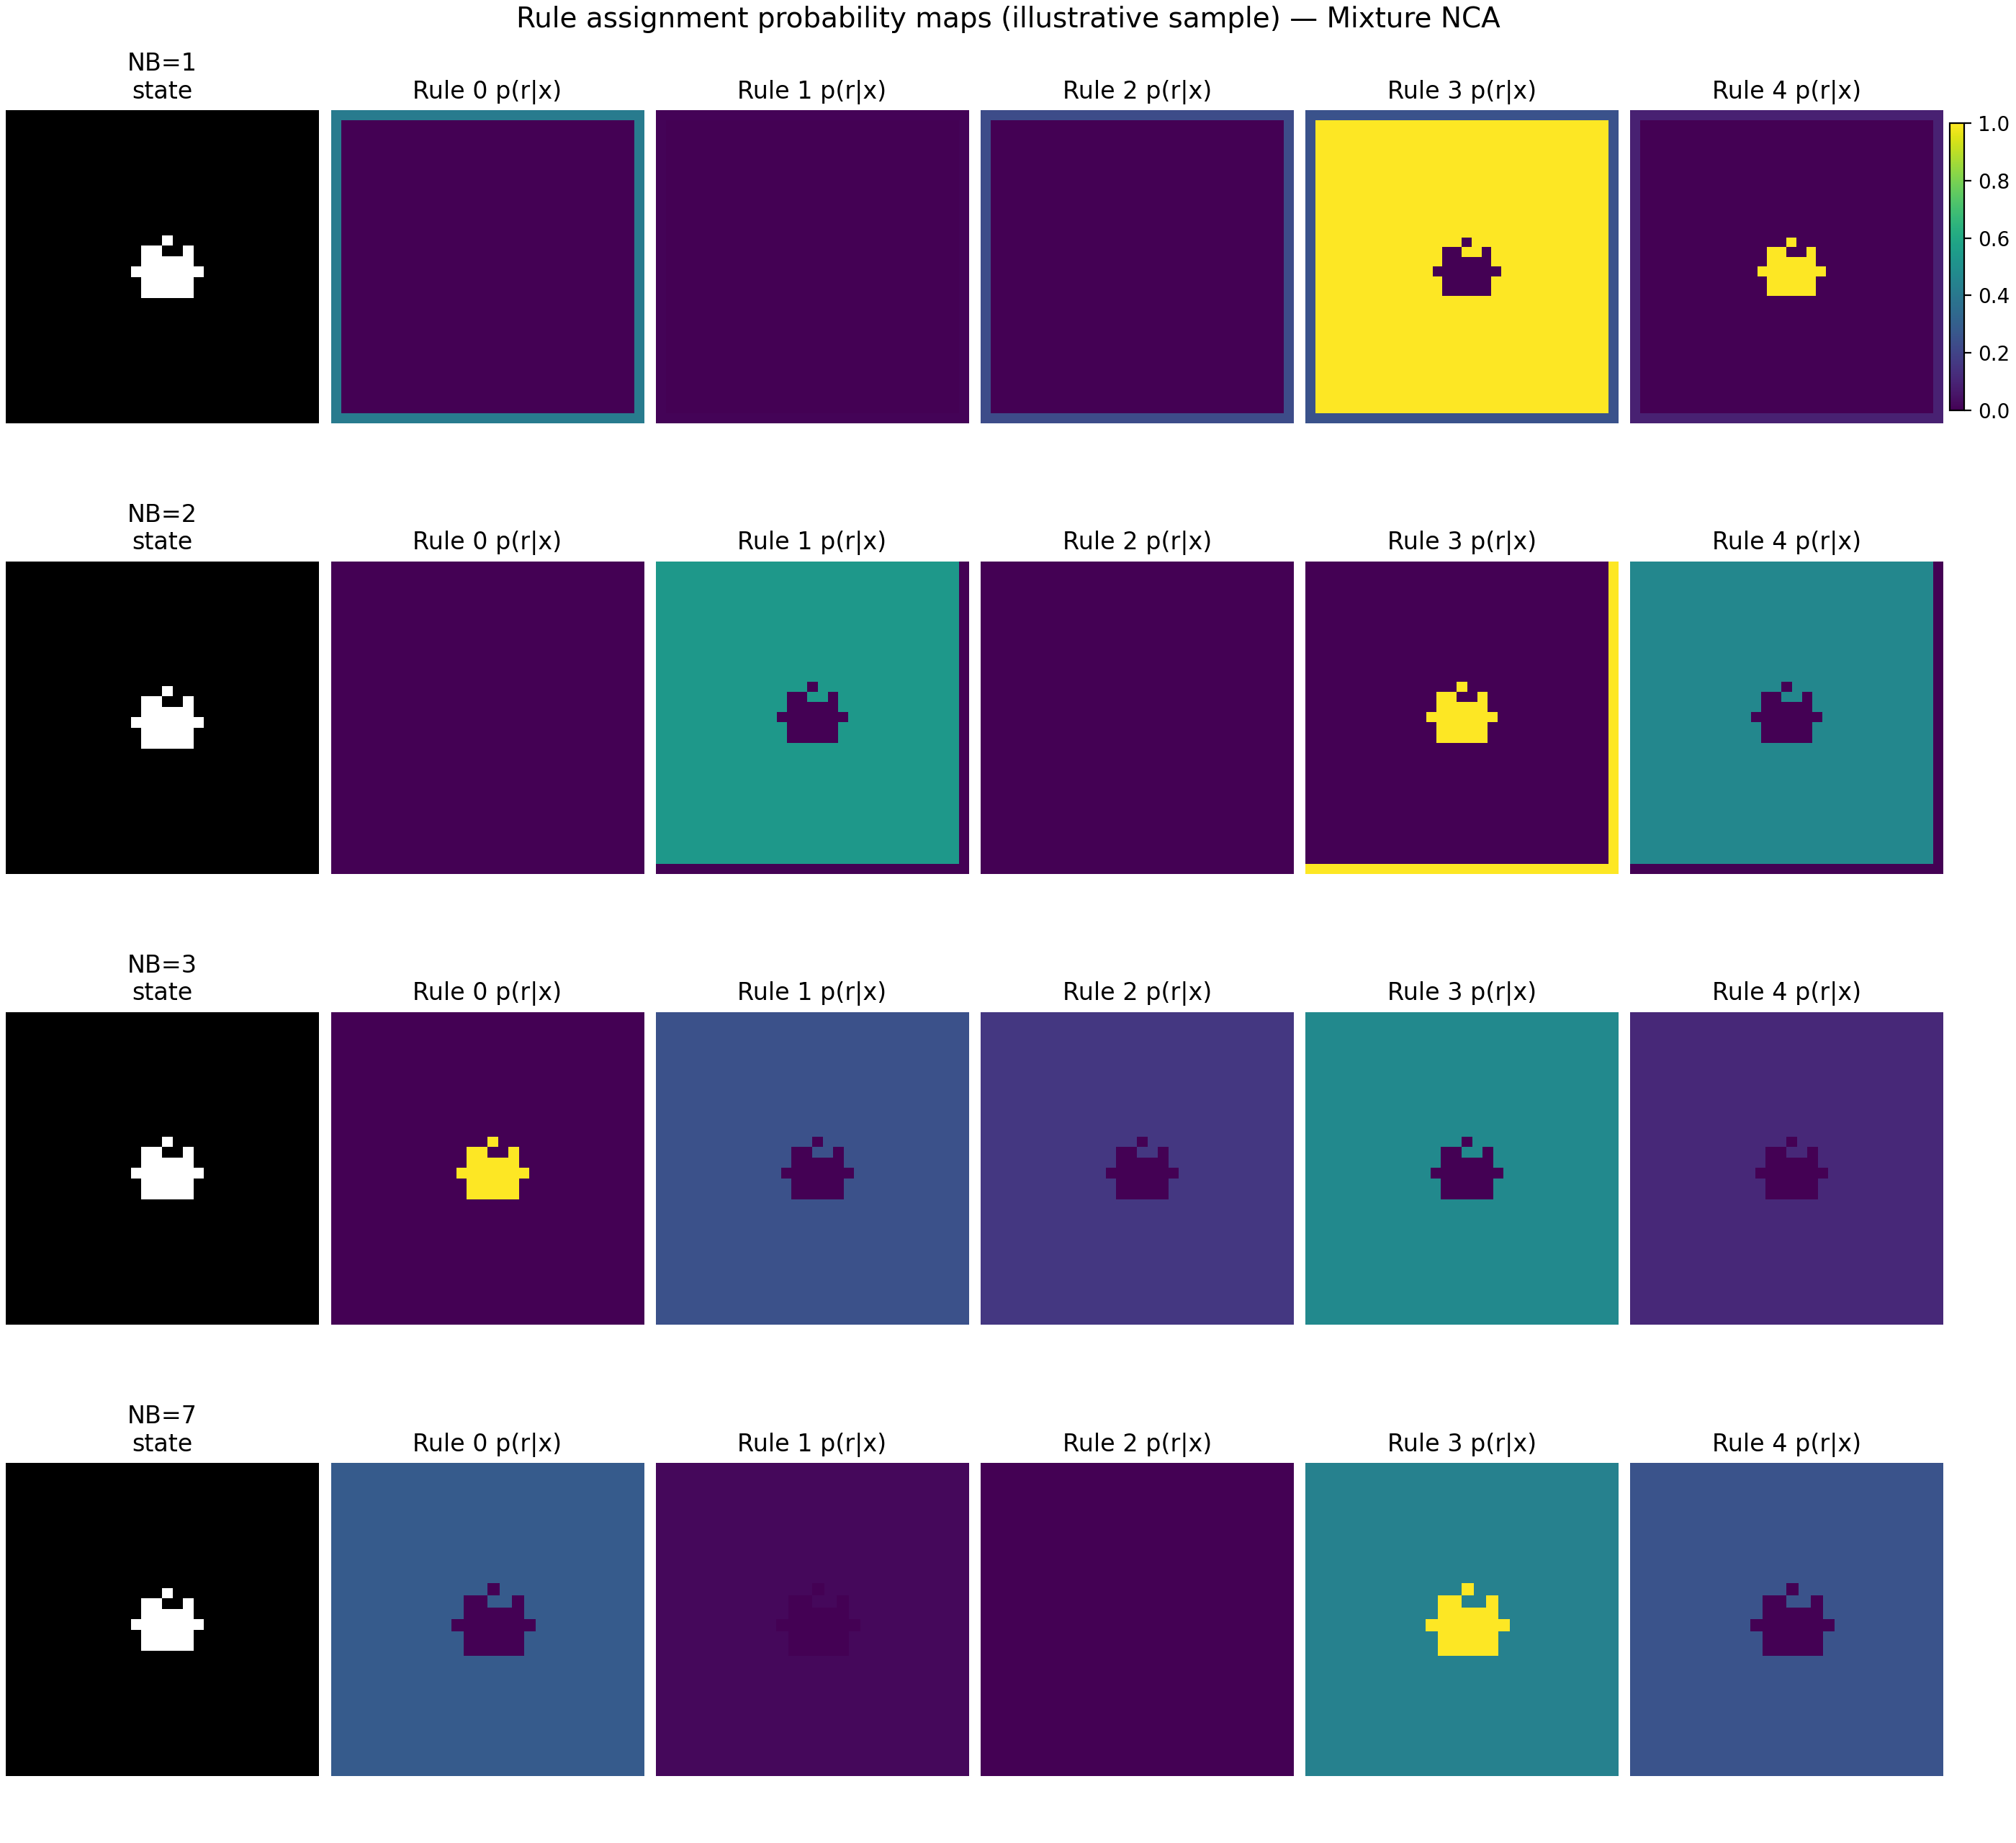
\includegraphics[width=\textwidth]{figs/neighborhood_analysis/nb_sweep_300x100/rule_assignment_maps_mixture.png}
  \caption{Where the Mixture model puts high probability on each rule (one state; rows = \(NB\)).}
  \label{fig:rule:maps:mix}
\end{figure}

\textbf{Interpretation.} Heatmaps show how \(NB\) changes where each rule is used. That can partly explain the performance gaps between \(NB\). For small \(NB\), rule maps may look noisier or less spatially coherent; for larger \(NB\), we often see clearer zones (e.g.\ one rule near the border, another in the bulk), which can help the model keep structure stable over time.

\begin{figure}[htbp]
  \centering
  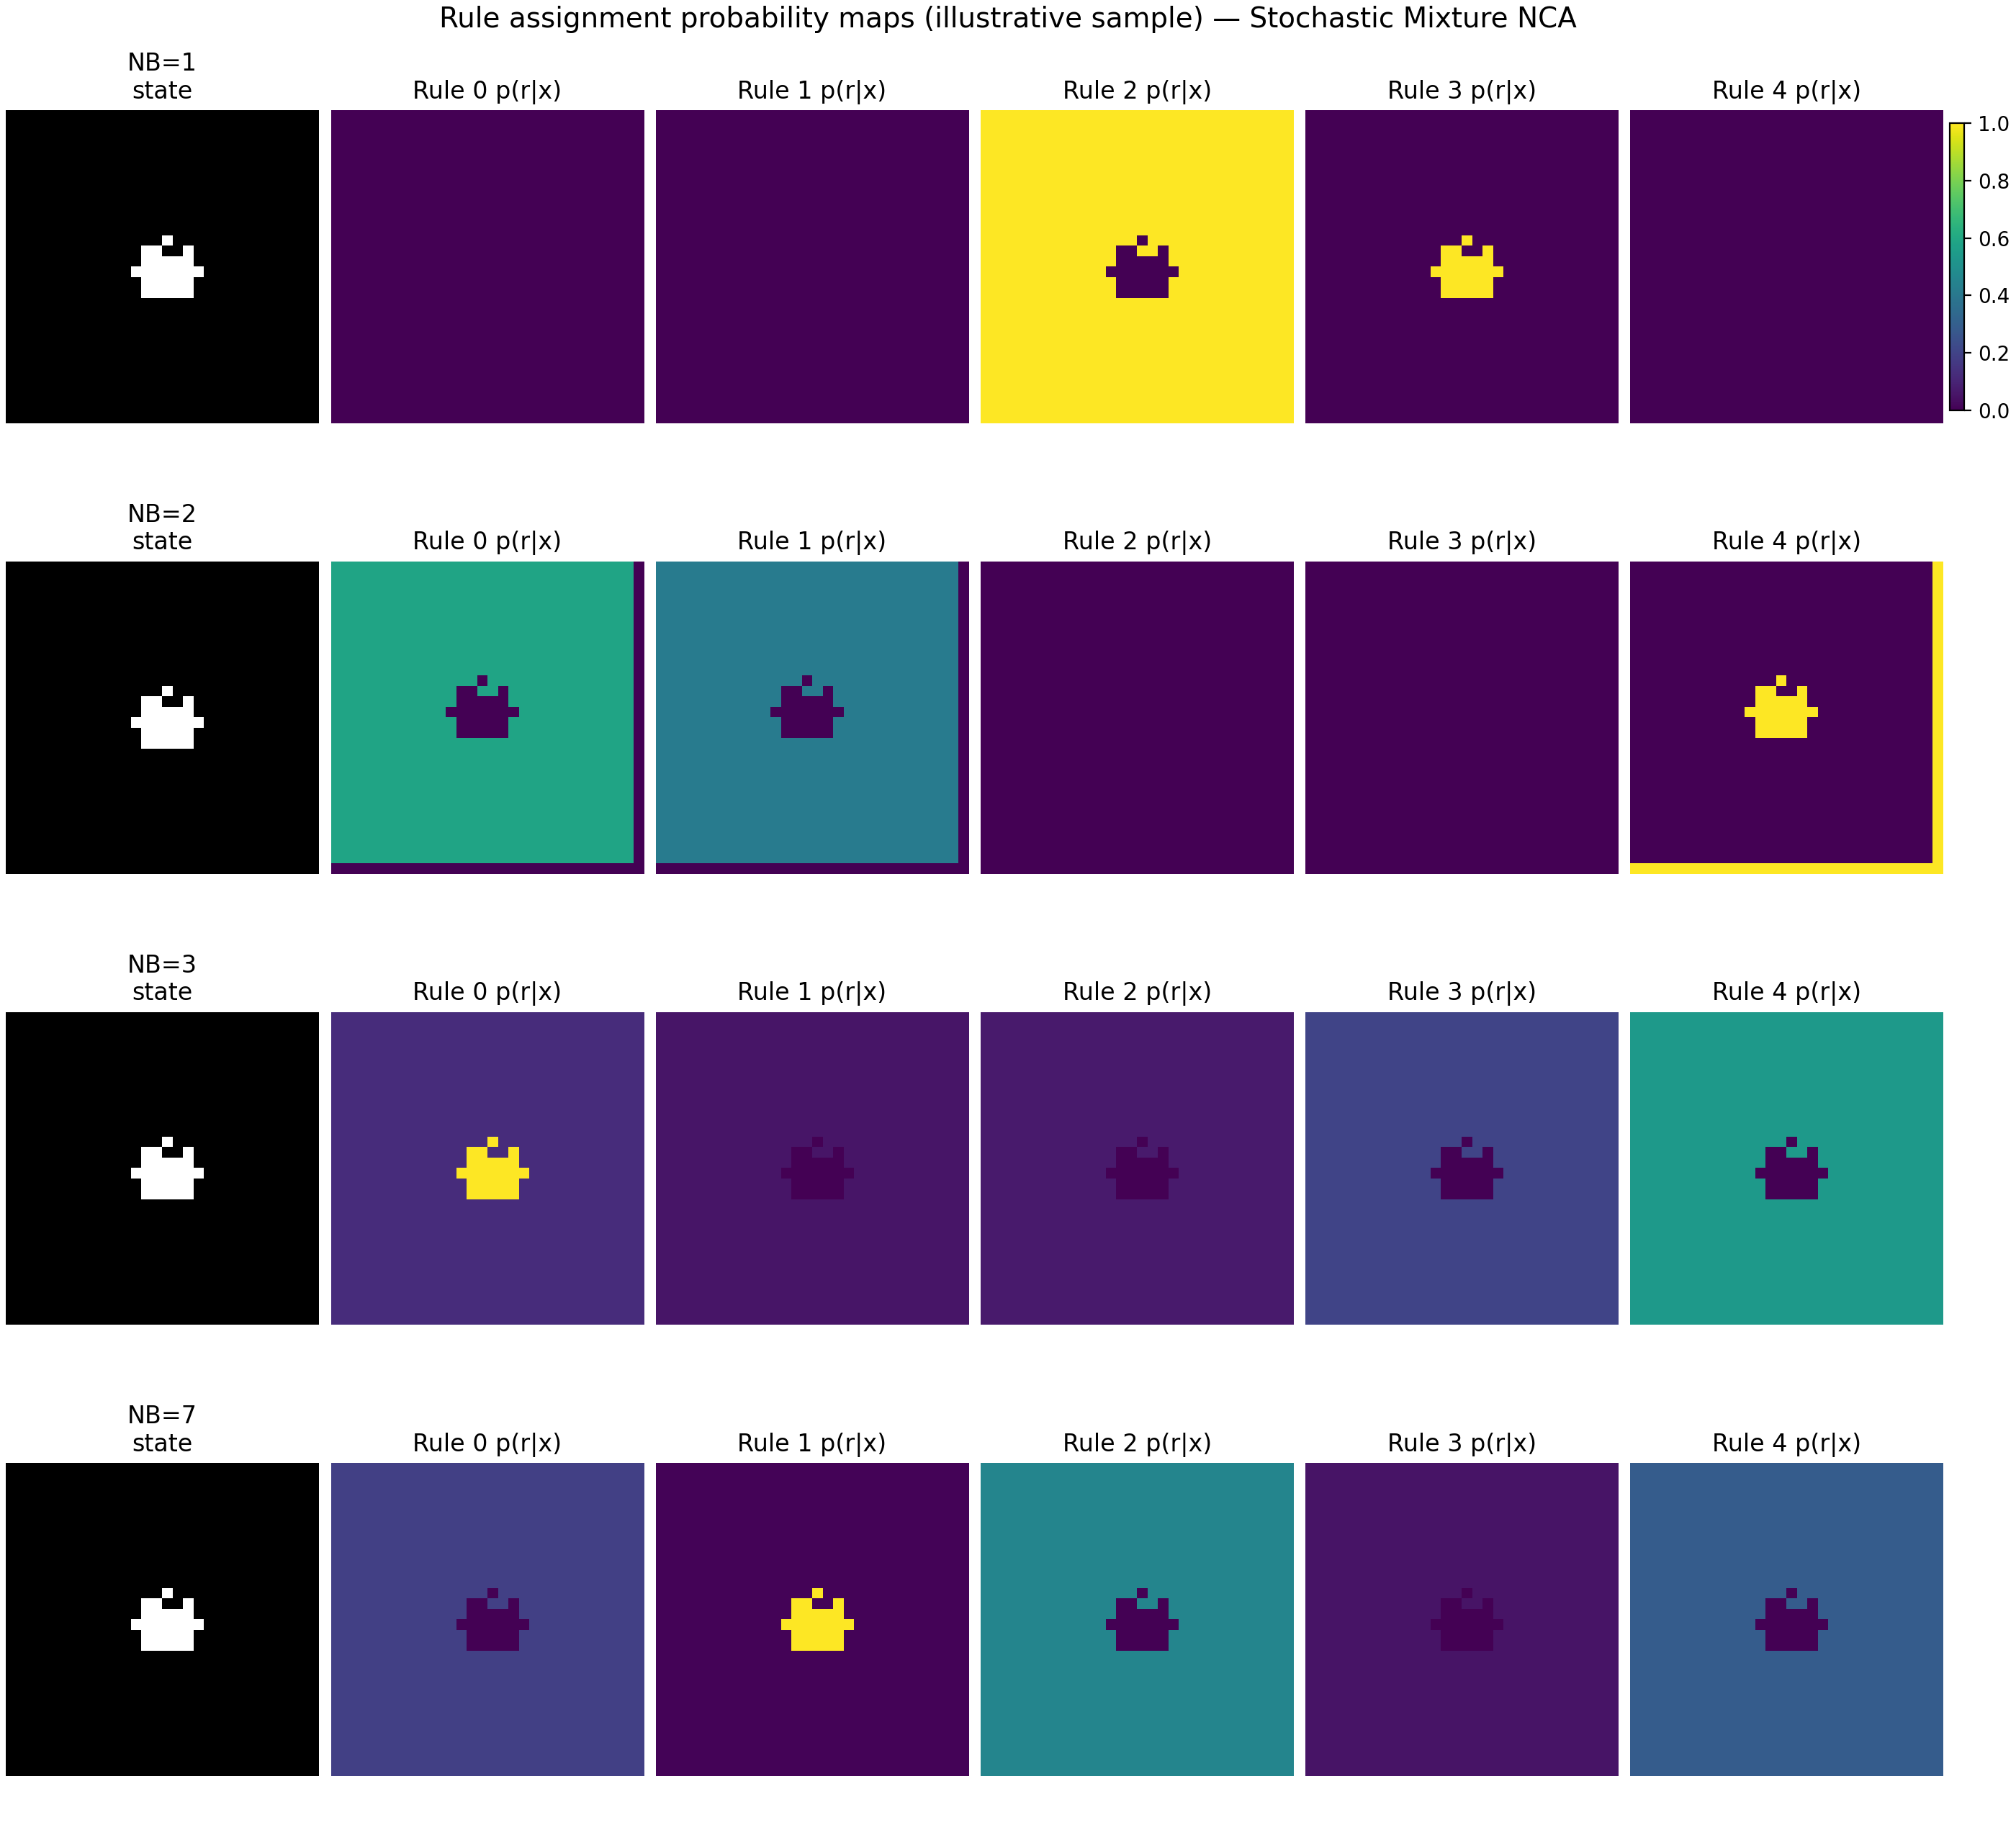
\includegraphics[width=\textwidth]{figs/neighborhood_analysis/nb_sweep_300x100/rule_assignment_maps_stochastic.png}
  \caption{Same for Stochastic Mixture (same state).}
  \label{fig:rule:maps:stoch}
\end{figure}

\textbf{Interpretation.} The stochastic model can have different spatial patterns of rule use even when average metrics are close, which fits with its different bad-rate and robustness. Comparing the two heatmaps (Mixture vs.\ Stochastic) for the same state and same \(NB\) shows where sampling makes rule use more or less concentrated in space, and that can help explain why the stochastic variant sometimes does better or worse on certain metrics.

%-------------------------------------------------------------------
\section{Statistical tests}
%-------------------------------------------------------------------

Metrics are heavy-tailed, so we use non-parametric tests: Kruskal--Wallis over all \(NB\), then Mann--Whitney U with Holm correction for two baselines---each \(NB>2\) vs.\ \(NB=2\), and each \(NB>3\) vs.\ \(NB=3\) (we do not compare against \(NB=1\), which is trivially inadequate).

\begin{table}[htbp]
\centering
\small
\resizebox{\textwidth}{!}{%
\begin{tabular}{@{}llccc@{}}
\toprule
Model & Metric & K-W $p$ & Significant vs.\ NB=2 & Significant vs.\ NB=3 \\
\midrule
Mixture NCA & KL Divergence & $<10^{-4}$ & 3,4,5,6,7 & 4,5,6,7 \\
Mixture NCA & Chi-Square & $<10^{-4}$ & 3,4,5,6,7 & 4,5,6,7 \\
Mixture NCA & Categorical MMD & $<10^{-4}$ & 3,4,5,6,7 & 4,5,6 \\
Mixture NCA & Tumor Size Diff & $<10^{-4}$ & 3,4,5,6,7 & 4,5,6,7 \\
Mixture NCA & Border Size Diff & $<10^{-4}$ & 3,4,5,6,7 & 4,5,6,7 \\
Mixture NCA & Spatial Variance Diff & $<10^{-4}$ & 3,4,5,6,7 & 4,5,6,7 \\
\midrule
Stochastic Mixture NCA & KL Divergence & $<10^{-4}$ & 3,4,5,6,7 & 4,5,6,7 \\
Stochastic Mixture NCA & Chi-Square & $<10^{-4}$ & 3,4,5,6,7 & 4,5,6,7 \\
Stochastic Mixture NCA & Categorical MMD & $<10^{-4}$ & 3,4,5,7 & 4,5,6,7 \\
Stochastic Mixture NCA & Tumor Size Diff & $<10^{-4}$ & 3,4,5,7 & 4,5,6,7 \\
Stochastic Mixture NCA & Border Size Diff & $<10^{-4}$ & 4,5,6,7 & 4,5,6,7 \\
Stochastic Mixture NCA & Spatial Variance Diff & $<10^{-4}$ & 3,4,5,6,7 & 4,5,7 \\
\bottomrule
\end{tabular}%
}
\caption{Step length = 100. Post-hoc (Holm-corrected): which \(NB>2\) differ from \(NB=2\), and which \(NB>3\) differ from \(NB=3\).}
\label{tab:stats}
\end{table}

\textbf{Interpretation.} The two baseline columns agree: the effect of \(NB\) is statistically significant. Compared to \(NB=2\), usually all of \(NB=3,4,5,6,7\) are significant (so even \(NB=3\) differs from the minimum); compared to \(NB=3\), we see which of \(NB=4,5,6,7\) differ from that reference---sometimes a subset (e.g.\ Categorical MMD or Spatial Variance) drops one of 6 or 7, meaning that larger \(NB\) is not always significantly better than \(NB=3\). The two baselines thus give a consistent and robust message: neighborhood size matters, and the ``best'' \(NB\) is metric- and model-dependent.

%-------------------------------------------------------------------
\section{Conclusions}
%-------------------------------------------------------------------

\begin{itemize}
\item Going from \(NB=1\) to \(NB\ge2\) gives a large gain in stability and scores for all metrics we use.
\item For \(NB\ge2\), scores do not always improve when we increase \(NB\); they depend on the metric and on rollout length. Some metrics get better with larger \(NB\), others get worse or stay flat.
\item To compare \(NB\) in a clear way, we need fixed sampling/temperature and several evaluation horizons (e.g.\ 25, 50, 100 steps).
\item Runtime per step is almost flat for \(NB\in[1,7]\), so using larger \(NB\) in this range does not cost much.
\end{itemize}

MNCA can model tissue-like dynamics in this synthetic setup. To get clear answers on \(NB\), we had to control training and evaluation (Step~3). When models already fail at long rollouts, the effect of \(NB\) is hard to see. Under the Step~3 protocol, the gain of \(NB\ge2\) and the dependence on metric and horizon are clear and backed by the plots and the statistical tests above.

\end{document}
